\documentclass{standalone}


\usepackage{tikz}
\usetikzlibrary{shapes,backgrounds,calc,patterns}
\usepackage{venndiagram}


\begin{document}
	     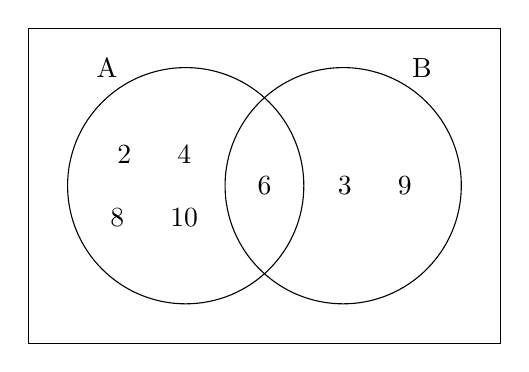
\begin{tikzpicture}
	\begin{scope} [fill opacity = 1]
	
	\draw (-3,2) rectangle (3,-2);
	
	\draw[draw = black] (-1,0) circle (1.5);
	\draw[draw = black] (1,-.0) circle (1.5);
	
	\node at (-2,1.5) {A};
	\node at (2, 1.5) {B};
	\node at (-1.4,.4) {2 \hspace{1em}   4};
	\node at (-1.4, -.4) {8 \hspace{1em}   10};
	\node at (1.4,0) {3 \hspace{1em}   9}; 
	\node at (0,0) {6};
	\end{scope}
	\end{tikzpicture}
\end{document}